We conducted several numerical experiments to confirm the validity of the error bounds formed in \cref{sec:mpanalysis}.
First, we tested \cref{algo:hhQR,algo:blockHQR,algo:par_tsqr,algo:mpBQR}, {\tt mpHQR2}, {\tt mpBQR2}, and {\tt mpTSQR2} for varying matrix sizes.
Then, we tested varying block sizes in \cref{algo:mpBQR} for a fixed matrix size, and lastly compared the performance of {\tt mpHQR2} and {\tt mpTSQR2}.
\subsection{Varying matrix sizes}
\subsection{Varying block sizes in {\tt mpBQR3}}
\subsection{Varying condition numbers and comparing {\tt mpHQR2} against {\tt mpTSQR2}}
\subsection{Numerical Experiment}
\label{sec:NE}
%\subsection{Single Precision}
In Section~\ref{sec:HTSQR}, we theorized that conditions exist where TSQR could outperform HQR and that these conditions were hard to identify in mixed-precision settings. 
An empirical comparison of these two QR factorization algorithms in double precision can be found in \cite{Mori2012}, where they conclude that deeper TSQR tends to produce more accurate QR factorizations than HQR.
However, using TSQR with deep levels (large $L$) can actually start to perform worse than TSQR with shallower levels (smaller $L$), since deeper levels require more FLOPs.
We instead focused on comparing HQR and TSQR performances in a mixed-precision setting.
Our numerical simulations show that TSQR can still outperform HQR in low, mixed-precision settings in practice even though the theoretical bounds do not guarantee stability.
%are all $\mathcal{O}(10)$ (c.f. Table~\ref{table:HTSQRerr}), and get larger as we go from HQR to TSQR, and larger as we increase $L$. 
Our empirical results do not behave as the theoretical bounds suggest, and even show opposite trends at times. 
This discrepancy highlights the shortcomings of deterministic error bounds that are too pessimistic. \par
%showed that there exists conditions in which the worst-case rounding error bound for TSQR can be expected to be smaller than that of HQR. 
%These conditions are met more easily in high, uniform-precision settings than low mixed-precision settings.
%The success of TSQR in high, uniform-precision settings is explored and discussed in \cite{Mori2012}, where they conclude that the computed relative error, $\|\hat{\bb{Q}}\hat{\bb{R}}-A\|_F$, tends to decrease as they increase $L$, but only up to a certain point.
%This may appear to contradict our conclusion in Section~\ref{sec:upHTSQR}, where we found that as long as $\frac{L}{2^{L-1}}\ll 1$, there e 
%\subsubsection{Experiment Details}
We used Julia v1.0.4 for all of the numerical simulations. 
This programming language allows half precision storage as well as {\tt castup} and {\tt castdown} operations to and from single and double precisions, but has no half precision arithmetic.
Therefore, we relied on using Algorithm~\ref{algo:simulate} for $f\in \text{OP} \cup\{{\tt dot\_product}\}$ to simulate half and mixed-precision arithmetic operations. 
%Specifically, we approximated , and 
%To simulate the mixed-precision setting described in Assumption~\ref{assump:mp} with $u_p = 0$ (which implies $z=1$), we used Algorithm~\ref{algo:simulate} for the dot product routine.
%That is, for $\bb{x}_{\text{half}},\bb{y}_{\text{half}}\in\F_{\text{half}}^m$, we approximated $\fl(\bb{x}_{\text{half}}^{\top}\bb{y}_{\text{half}})$ with {\tt simHalf}$(${\tt dot\_product} $, \bb{x}_{\text{half}}, \bb{y}_{\text{half}})$ to simulate mixed-precision dot products.
%We used Algorithm~\ref{algo:simulate} for all other operations as well to simulate half precision arithmetic.
For HQR, we created a mixed-precision version of the LAPACK routine xGEQRF, where the dot product subroutine was approximated by $\fl(\bb{x}_{\text{half}}^{\top}\bb{y}_{\text{half}})$ with {\tt simHalf}$(${\tt dot\_product} $, \bb{x}_{\text{half}}, \bb{y}_{\text{half}})$ to simulate the mixed-precision setting described in Assumption~\ref{assump:mp} with $u_p = 0$ (which implies $z=1$), and we used Algorithm~\ref{algo:simulate} on all other basic operations in OP to simulate half/storage precision arithmetic. 
%Using these simulated operations as subroutines for 
%By using these simulated half and mixed precision versions of basic operations at subroutines for our implementation of the LAPACK routine xGEQRF, we 
%To implement half and mixed-precision simulations within HQR, we wrote our own versions of it that almost replicates LAPACK routine xGEQRF, where the disparity only comes from the storage format of the information required to build the $\bb{Q}$ factor. 
This HQR was then used as a subroutine of TSQR as well. 
There are cases where the rounding will differ between the mixed-precision setting and the way we mimic it, i.e., basic operations that are meant to be in half/storage precision arithmetic, but are instead casted up to single and back down, as the tiebreaker within correct rounding may lead to different results than true half/storage precision arithmetic. 
All in all, our experiments nearly replicated the mixed-precision setting we assumed for the error analysis in Sections~\ref{sec:HQRre} and \ref{sec:TSQRre}.\par 
%Although we kept the matrix size constant, we varied the condition numbers of these matrices by the method described below.
%We speculated that matrices with larger condition numbers would behave closer to the ``worst-case scenario'' with respect to rounding errors.
%Table~\ref{table:HTSQRerr} shows the theoretical error bounds from Section~\ref{sec:HQRre} and \ref{sec:TSQRre} that correspond to the conditions of our experiment.
%Stability is not guaranteed for any of these QR factorization methods. 
%
%\begin{table}[h]
%	\centering
%	\begin{tabular}{||c|c|c|c|c|c|c|c||} 
%		\hline
%		$L$ & $0$ & $1$ & $2$ & $3$ & $4$ & $5$ & $6$ \\ \hline
%		$n^{3/2}(\gamma_w^{(6d_1+ 25)}+L\gamma_w^{(6d_2+ 25)})$ & {\tt 9.36} & {\tt 18.73} & {\tt 28.09} & {\tt 37.46} & {\tt 46.82} & {\tt 56.19} & {\tt 65.55}\\ \hline
%	\end{tabular}
%	\caption{Error bounds for when $m=4000$, $n=100$, $u_w=u_{\text{half}}$, $u_s={\text{single}}$, and $d_1,d_2$ are defined in Section~\ref{sec:TSQRre}. Error bound for HQR is recovered when $L=0$.}
%	\label{table:HTSQRerr}
%\end{table}

%\paragraph{Constructing Test Matrices}
Following example from \cite{Mori2012}, we used $m$-by-$n$ random matrices, $\bb{A}_{\alpha}$, constructed via
\begin{equation}
\bb{A}_{\alpha} = \bb{Q'}(\alpha \bb{E} + \bb{I})/\|\bb{Q'}(\alpha \bb{E} + \bb{I})\|_F,
\label{eqn:genRM}
\end{equation}
where $\bb{Q'}\in\mathbb{R}^{m\times n}$ is a random orthogonal matrix and $\bb{E}\in\R^{n\times n}$ is the matrix of $1$'s. 
The random orthogonal matrix $\bb{Q'}$ is generated by taking a QR factorization of an iid $4000$-by-$100$ matrix sampled from $Unif(0,1)$, and we used the built-in QR factorization function in Julia.
By construction, $\bb{A}_{\alpha}$ has 2-norm condition number $n\alpha+1$. 
By varying $\alpha$ from {\tt 1e-4} to {\tt 1}, we varied the condition number from $1.1$ to $101$, and we generated $10$ samples for each value of $\alpha$.

%\subsubsection{Results}


We generated random matrices of size $4000$-by-$100$ using Equation~\ref{eqn:genRM} and computed their HQR and TSQR for $L=1, \cdots, 6$ in a mixed-precision setting that simulates Assumption~\ref{assump:mp} with $z=1$.
The relative backward error, $\|\hat{\bb{Q}}\hat{\bb{R}}-\bb{A}\|_F/\|\bb{A}\|_F$, was computed by casting up $\hat{\bb{Q}}$, $\hat{\bb{R}}$, and $\bb{A}$ to double precision to compute the Frobenius norms.
Note that the mixed-precision HQR error bounds $n\tilde{\gamma}_{w}^{(6d+6z+13)}$ and $n^{3/2}\tilde{\gamma}_{w}^{(6d+6z+13)}$ for $m=4000$ and $n=100$ are {\tt 0.936} and {\tt 9.364} respectively, and the mixed-precision TSQR bounds for $L=1,\cdots, 5$  are even larger, which indicates that our error bounds do not guarantee stability.\par

\begin{wrapfigure}{l}{.4\textwidth}
	\centering
	\vspace{-10pt}
	\includegraphics[width=.4\textwidth]{./figures/unblocked.pdf}
	\caption{\label{fig:unblocked} HQR errors for matrices with varying condition numbers.}
	%\vspace{-10pt}	
\end{wrapfigure}
Figure~\ref{fig:unblocked} shows the backward errors of mixed precision HQR increasing as the theoretical condition numbers of the generated random matrices increase, and these errors correspond to the error data on the vertical axis, $L=0$, of Figure~\ref{fig:allTSQR}.
In addition to the errors from HQR, Figure~\ref{fig:allTSQR} shows the errors from mixed precision TSQR of levels varying from $L=1$ to $L=5$, where each line represents the errors of HQR and variants of TSQR calculated from the same random test matrix.
Figure~\ref{fig:allTSQR} reveals two different trends for the errors as we deepen the complexity of the QR algorithm from HQR to TSQR with 5 levels. 
One trend occurs for matrices with smaller condition numbers, where HQR and all levels of TSQR are stable, but deepening the levels of TSQR worsens the errors. 
The other trend occurs for matrices with higher condition numbers, where single-level and 2-level TSQR yield smaller errors than HQR. 
In these cases, TSQR with 3 or more levels have errors similar to or worse than 2-level TSQR, but those errors tend to not rise above the HQR errors.
These results suggests that TSQR can significantly outperform HQR even in mixed-precision settings, and particularly when HQR is unstable due to larger condition numbers.
Although this experiment focused on condition numbers, identifying other properties that point to better performance of TSQR than HQR can further broaden the potential use of mixed-precision TSQR in applications.
%The first trend When the error is low enough for the unblocked QR factorization, TSQR performs worse for these matrices.
%Recall that machine precision for half-precision is about $10^{-3}$. 
%This shows that the traditional QR factorization had been very good to begin with.
%Finally, even when TSQR is \textit{successful} initially, we can see that too many initial blocks can become a problem as well. 
%
%Overall, this figure shows a variety of results that encourage further exploration. 
%We have shown that TSQR can improve on certain matrices where the unblocked HQR algorithm was highly unstable in half-precision.
%Identifying which matrix properties correlate to TSQR and why can help broaden the possibility of using lower precision arithmetic for QR factorizations.

\begin{figure}[h!]%{r}{.53\textwidth}
	\centering
	%\vspace{-10pt}
	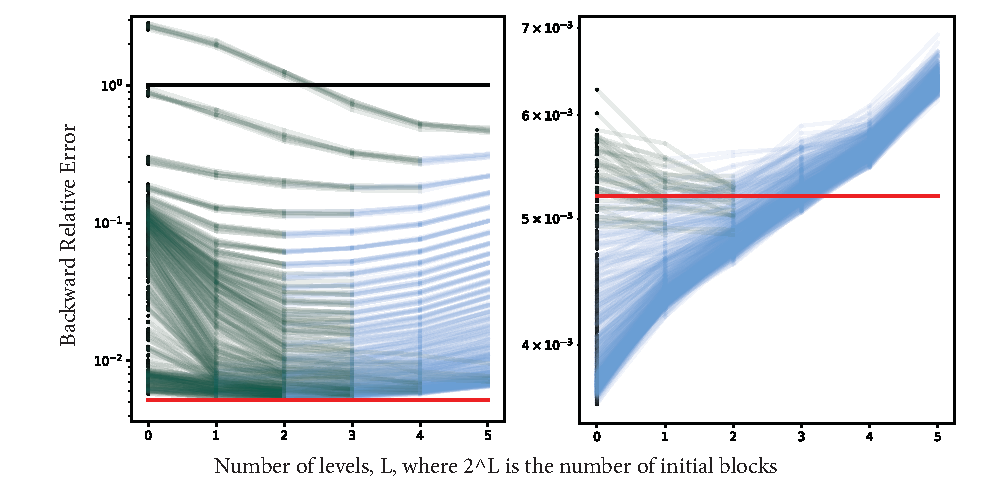
\includegraphics[width=0.8\textwidth]{./figures/allTSQR2.pdf}
	\caption{\label{fig:allTSQR} Left plot shows the relative error of QR factorization for matrices with condition numbers ranging from 5.3 to 101, and the right plot shows the errors for matrices with condition numbers ranging from 1.1 to 5.3. }
	\vspace{-10pt}
\end{figure} 
